\documentclass{beamer}
\usepackage{multicol}

\usepackage{clrscode3e}
\usepackage{amsmath,amsfonts}
\usepackage{graphicx,color}

\newcommand{\bi}{\begin{itemize}}
\newcommand{\ii}{\item}
\newcommand{\ei}{\end{itemize}}
\newcommand{\bn}{\begin{enumerate}}
\newcommand{\en}{\end{enumerate}}
\newcommand{\set}[1]{\ensuremath{\left\{#1\right\}}}
\newcommand{\pr}[1]{\ensuremath{\mbox{Pr}\left\{#1\right\}}}
\newcommand{\flr}[1]{\ensuremath{\left\lfloor#1\right\rfloor}}
\newcommand{\ceil}[1]{\ensuremath{\left\lceil#1\right\rceil}}

\newcommand{\sect}[1]{
\section{#1}
\begin{frame}[fragile]\frametitle{#1}
}


\setlength{\tabcolsep}{4\tabcolsep}

\newcommand{\nop}[1]{}

\newcommand{\att}[2]{\attrib{#1}{#2}}
\newcommand{\attt}[3]{\attrib{\attrib{#1}{#2}}{#3}}
\newcommand{\atttt}[4]{\attrib{\attrib{\attrib{#1}{#2}}{#3}}{#4}}


\title{Notes on Red-black Trees}
\author{Geoffrey Matthews}
\begin{document}
\begin{frame}
  \maketitle
\end{frame}


\sect{Red-black trees}
\bi
\ii A variation of binary search trees.
\ii \textbf{Balanced:} height is $O(\lg n)$, where $n$ is number of nodes.
\ii Operations will take $O(\lg n)$ in worst case.
\ei

\end{frame}

\sect{Red-black trees}
\bi
\ii A \textbf{red-black tree} is a binary search tree.
\ii One bit per node stores an attribute \textit{color}, red or black.
\ii All leaves are empty (nil) and colored black.
\ii We use a sentinel $\attrib{T}{nil}$ for all the leaves of a
red-black tree $T$.
\ii $\attrib{\attrib{T}{nil}}{color}$ is black.
\ii The root's parent is also $\attrib{T}{nil}$.
\ei


\end{frame}

\sect{Red-black tree properties}

\begin{enumerate}
  \ii Every node is either red or black.
  \ii The root is black.
  \ii Every leaf ($\attrib{T}{nil}$) is black.
  \ii If a node is red, then both its children are black

  Hence no two reds in a row.
  \ii For each node, all paths from the node to descendant leaves
  contain the same number of black nodes.
\end{enumerate}
\end{frame}

\sect{Red-black tree}

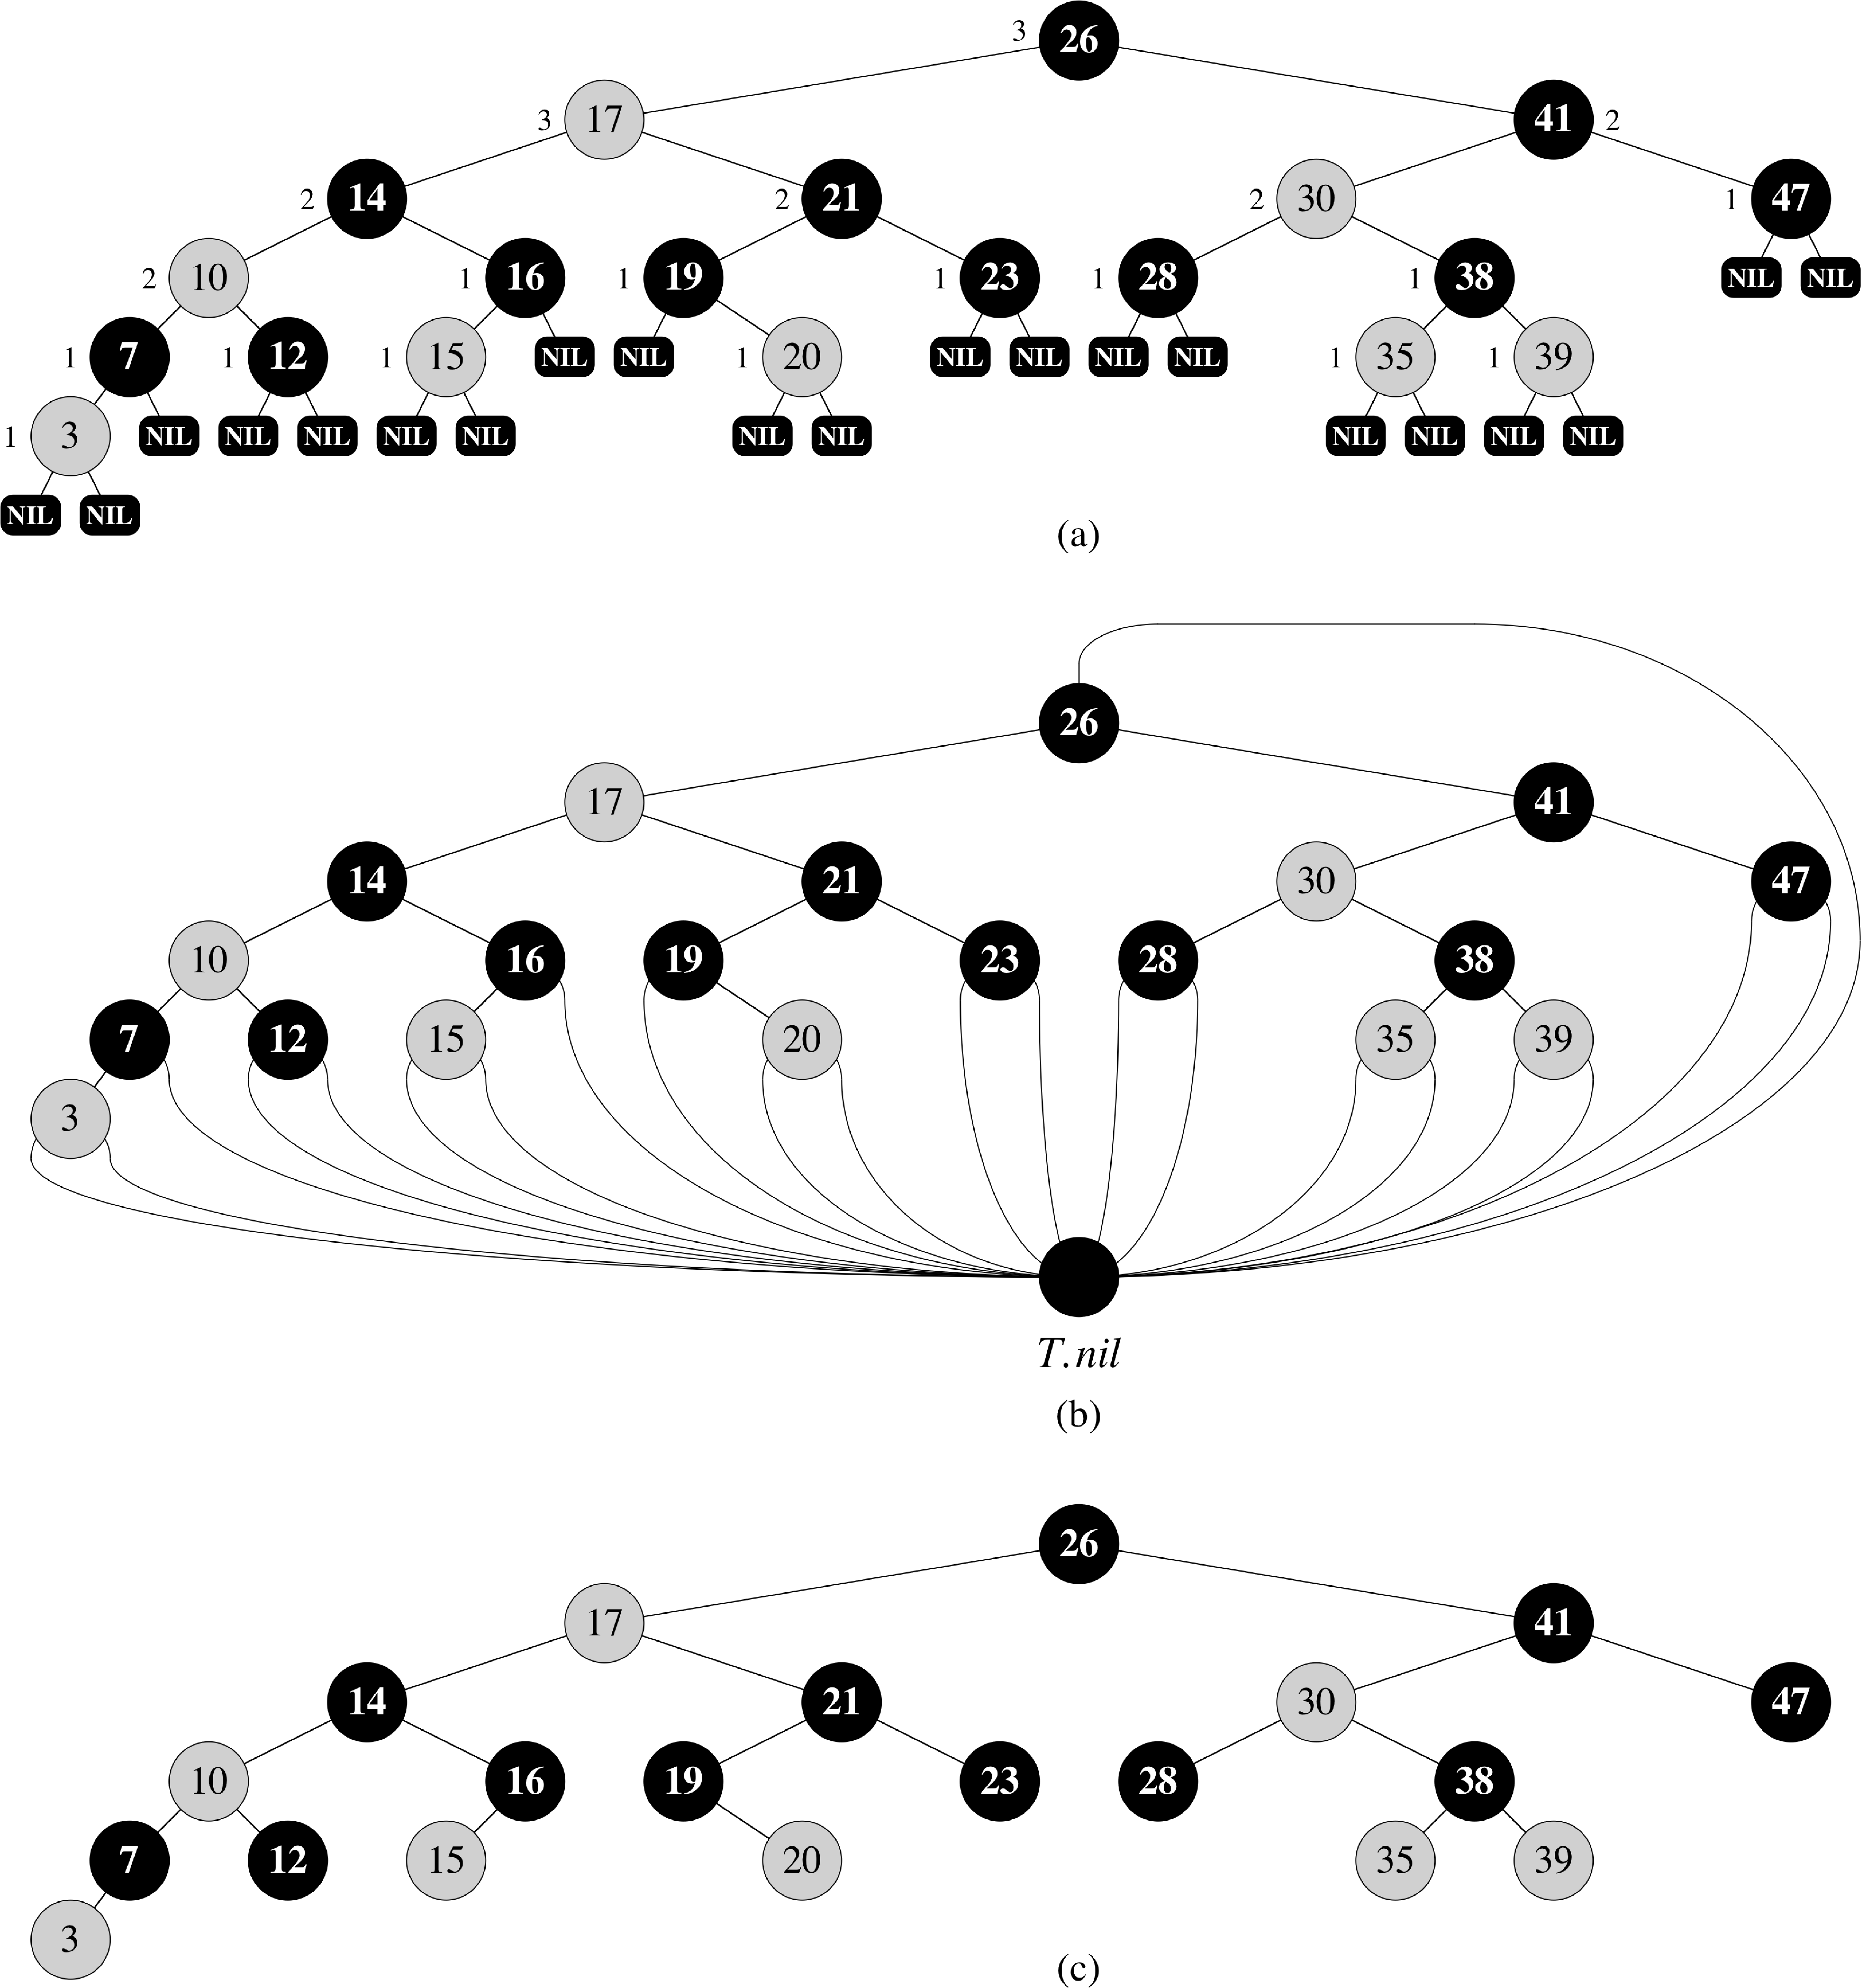
\includegraphics[height=0.8\textheight]{Fig-13-1.pdf}

\end{frame}

\sect{Height of a red-black tree} \bi \ii \textbf{Height of a node} is
the number of edges in longest path to leaf.  \ii
\textbf{Black-height} of a node $x$: bh($x$) is the number of black
nodes (including $\attrib{T}{nil}$) on a path from $x$ to a leaf, not
counting $x$.  \bi \ii By property 5, black-height is well defined.
\ii Changing the color of a node does not change its black-height.
\ii Changing the color of a node will change the black-height of its
ancestors.  \ei

\ei

\end{frame}

\sect{Claim 1:} Any node with height $h$ has black-height $\geq h/2$.

\bigskip

  \textbf{Proof}
\bi\ii
  By property 4, $\leq h/2$ nodes on the path from node to a leaf are
  red.\ii  Hence $\geq h/2$ are black.\ei

\end{frame}

\sect{Claim 2:} The subtree rooted at $x$ contains $\geq
  2^{\id{bh}(x)}   - 1$ internal nodes.

\bigskip
  
\textbf{Proof.}  By induction on height of $x$.

\textbf{Basis:} Height of $x=0\Rightarrow x$ is a leaf and so
$\id{bh}(x)=0$, $2^0-1=0$.

\textbf{Inductive step:}
\bi
\ii Let the height of $x$ be $h$.
\ii Any child of $x$ has height $h-1$ and black-height
either $bh(x)$ (if the child is red) or $bh(x)-1$ (if the child is black).
\ii By
inductive hypothesis, each child has $\geq 2^{\id{bh}(x)-1}-1$
internal nodes. \ii
Thus, the subtree rooted at $x$ contains $\geq 2\cdot
(2^{\id{bh}(x)-1}-1) + 1 = 2^{\id{bh}(x)}-1$ internal nodes.
\ei  

\end{frame}

\sect{Lemma:} A red-black tree with $n$ internal nodes
and height $h$ has
  \[
  h\leq 2\lg (n+1)\]

\bi\ii Recall proven claims:
\bi
\ii  Any node with height $h$ has black-height $\geq h/2$.
\ii  The subtree rooted at any node $x$ contains $\geq
  2^{\id{bh}(x)}   - 1$ internal nodes.
\ei\ei

\textbf{Proof}

 Let $h$ and $b$ be the height and black-height of the root,
 respectively.
 
 By the above two claims,
\[ n \geq 2^b-1 \geq 2^{h/2} - 1 \]
Adding 1 to both sides and then taking logs gives
\[ \lg(n+1) \geq h/2\]
which implies that
\[
h \leq 2\lg(n+1)
\]


\end{frame}

\sect{Operations on red-black trees}
\bi
\ii $\proc{Minimum}$, $\proc{Maximum}$, $\proc{Successor}$,
$\proc{Predecessor}$ and $\proc{Search}$ all run in $O(h) = O(\lg n)$
time.
\ii $\proc{Insert}$, what color to make the new node?
\bi \ii Red?
\bi\ii Might violate property 4.\ei
\ii Black?
\bi\ii Might violate property 5.\ei
\ei
\ii $\proc{Delete}$, what color was the old node?
\bi
\ii Red?  OK.
\bi\ii Unless successor is black?\ei
\ii Black?
\bi\ii Could cause two reds in a row, and violate properties 2 and 5.\ei
\ei
\ei

\end{frame}

\sect{Rotations}

\bi
\ii Only pointers are changed.
\ii Won't upset binary-search-tree property.
\ii Doesn't care about red-black.
\ei

\begin{multicols}{2}
\begin{codebox}
  \Procname{$\proc{Left-Rotate}(T,x)$}
  \li $y \gets \attrib{x}{right}$
  \li $\attrib{x}{right} \gets \attrib{y}{left}$
  \li \If $\attrib{y}{left}\not = \attrib{T}{nil}$ \Do
  \li $\attrib{\attrib{y}{left}}{p} \gets x$ \End
  \li $\attrib{y}{p} \gets \attrib{x}{p}$
  \li \If $\attrib{x}{p} \isequal \attrib{T}{nil}$ \Do
  \li  $\attrib{T}{root} \gets y$ 
  \li \ElseIf $x \isequal \attrib{\attrib{x}{p}}{left}$ \Do
  \li $\attrib{\attrib{x}{p}}{left} \gets y$
  \li \Else $\attrib{\attrib{x}{p}}{right} \gets y$ \End
  \li $\attrib{y}{left} \gets x$
  \li $\attrib{x}{p} \gets y$
\end{codebox}
\columnbreak
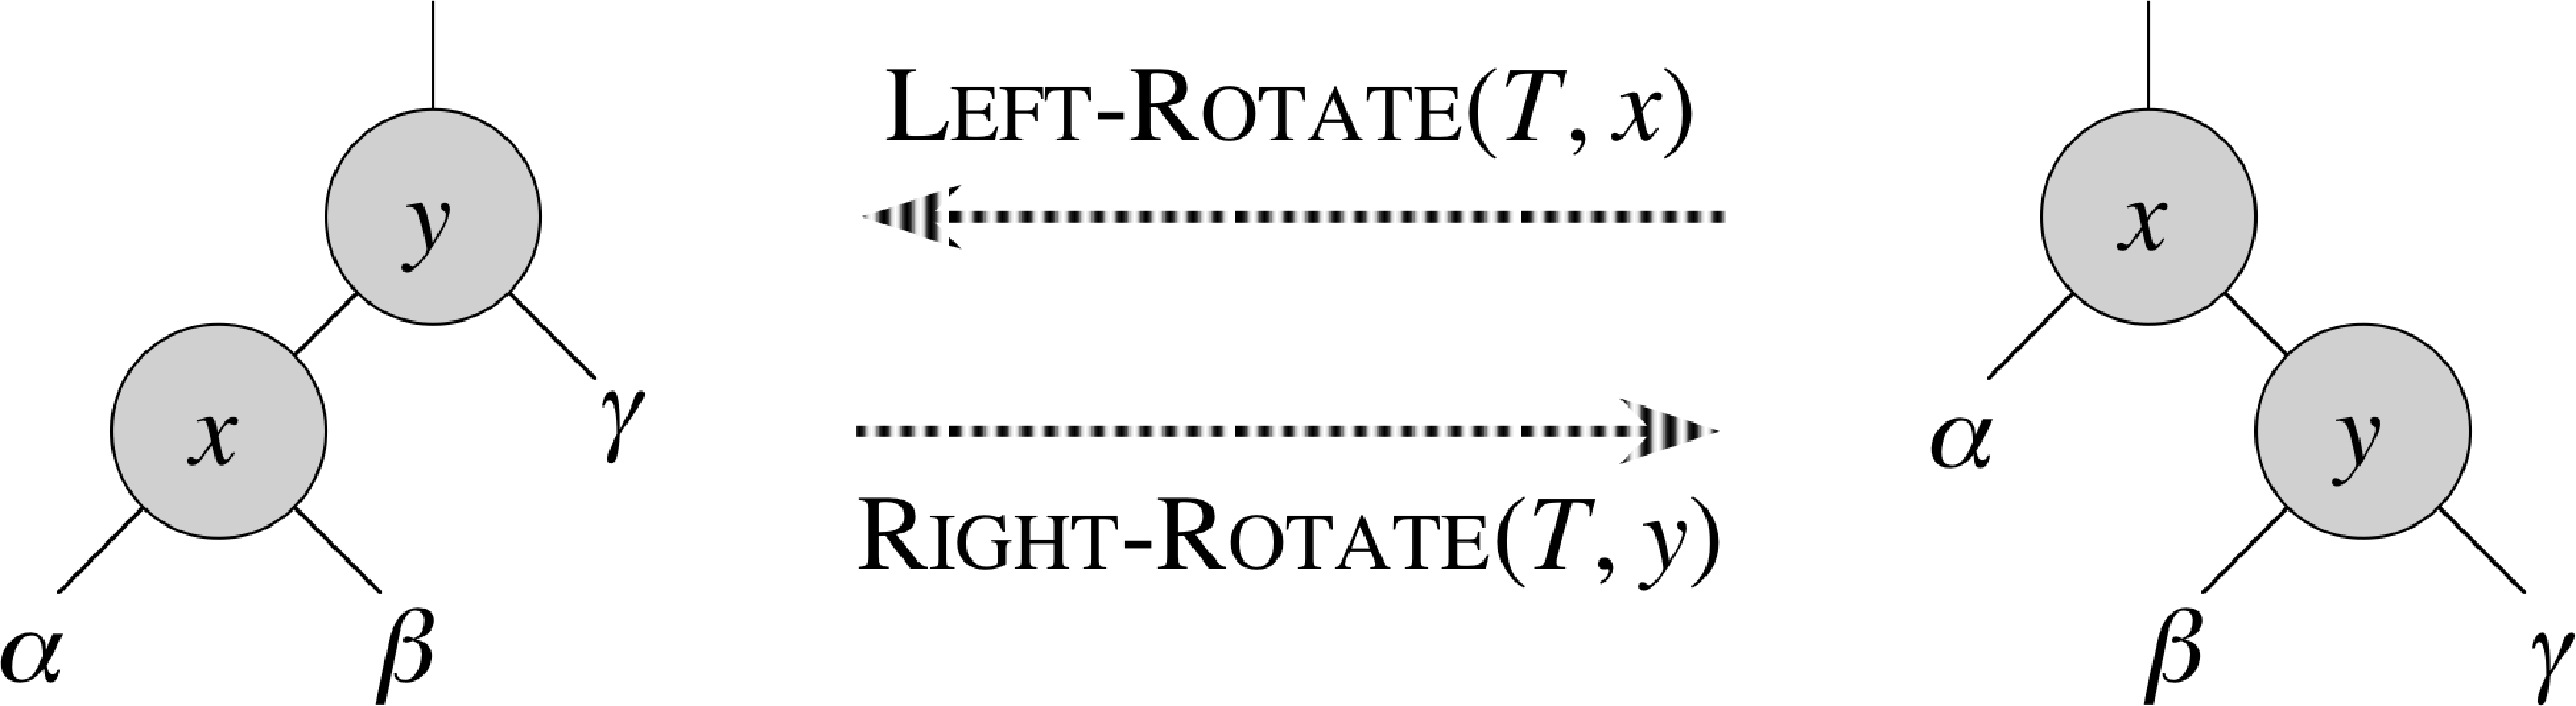
\includegraphics[width=0.5\textwidth]{Fig-13-2.pdf}

\vfill

 Assumes
\bi
\ii $\attrib{x}{right}\not = \attrib{T}{nil}$
\ii root's parent is $\attrib{T}{nil}$
\ei

\end{multicols}

\end{frame}
\sect{Rotations}

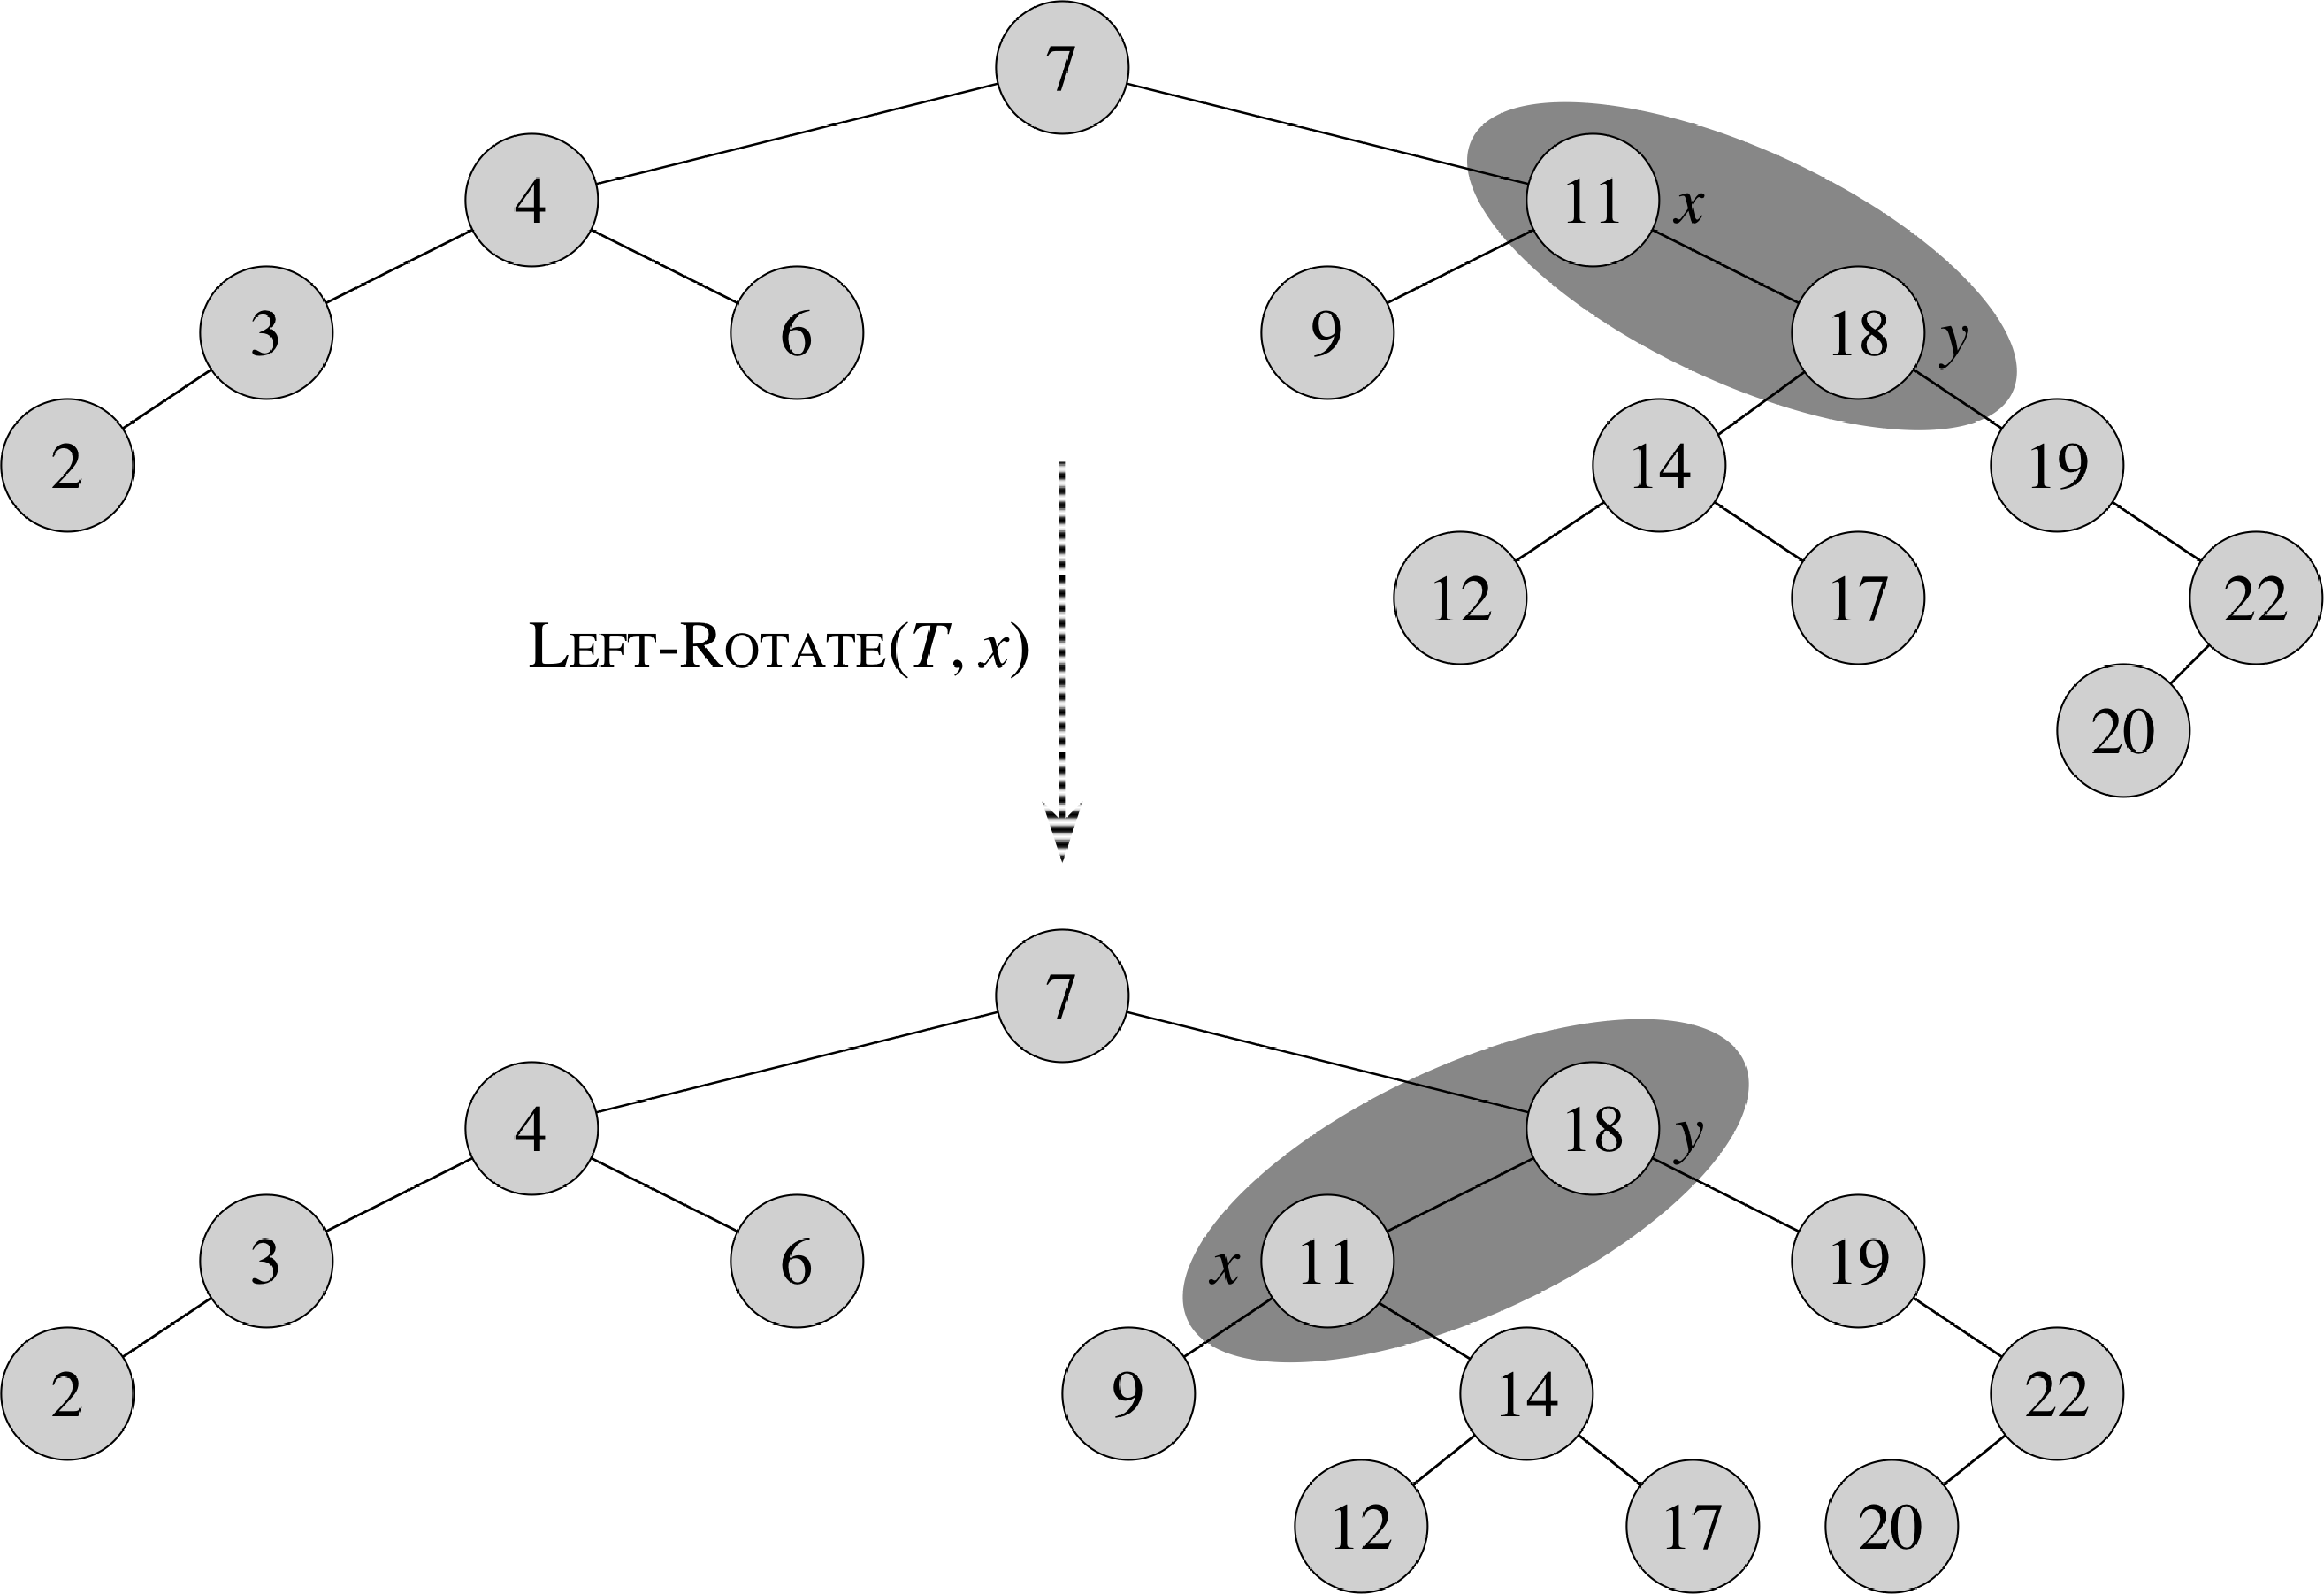
\includegraphics[width=\textwidth]{Fig-13-3.pdf}

\end{frame}

\sect{Insertions}
\scriptsize
\begin{multicols}{2}
\bi
\ii Start by doing regular binary-tree insertion.
\ii Color new node red.
\ii May violate red-black tree properties:
\ei

\begin{enumerate}
  \ii Every node is either red or black.

  OK.
  \ii The root is black.

  New node might be root.
  \ii Every leaf ($\attrib{T}{nil}$) is black.

   OK.
  \ii If a node is red, then both its children are black.
  
  New node's parent might be red.
  \ii For each node, all paths from the node to descendant leaves
  contain the same number of black nodes.

  OK.
\end{enumerate}

\columnbreak

\begin{codebox}
  \Procname{$\proc{RB-Insert-Fixup}(T,z)$}
  \li \While $\attrib{\attrib{z}{p}}{color} \isequal \const{red}$\Do
  \li \If $\attrib{z}{p} \isequal
  \attrib{\attrib{\attrib{z}{p}}{p}}{left}$ \Do
  \li $y \gets \attrib{\attrib{\attrib{z}{p}}{p}}{right}$
  \li \If $\attrib{y}{color} \isequal \const{red}$\Do 
  \li $\attrib{\attrib{z}{p}}{color} \gets \const{black}$
  \RComment{\color{red} case 1}
  \li $\attrib{y}{color}\gets \const{black}$
  \li $\attrib{\attrib{\attrib{z}{p}}{p}}{color} \gets \const{red}$
  \li $z\gets\attrib{\attrib{z}{p}}{p}$
  \li \Else \If $z\isequal\attrib{\attrib{z}{p}}{right}$ \Do
             \li $z\gets\attrib{z}{p}$ \RComment{ \color{red} case 2}
             \li $\proc{Left-Rotate}(T,z)$ \End
  \li $\attrib{\attrib{z}{p}}{color} \gets \const{black}$
  \RComment{\color{red} case 3}
  \li $\attrib{\attrib{\attrib{z}{p}}{p}}{color} \gets \const{red}$
  \li $\proc{Right-Rotate}(T,\attrib{\attrib{z}{p}}{p})$
\End
  \li \Else \li (``right'' $\rightleftharpoons$ ``left'') \End
\End
  \li $\attrib{\attrib{T}{root}}{color} \gets \const{black}$
\end{codebox}
\end{multicols}
\end{frame}

\sect{RB-Insert-Fixup}

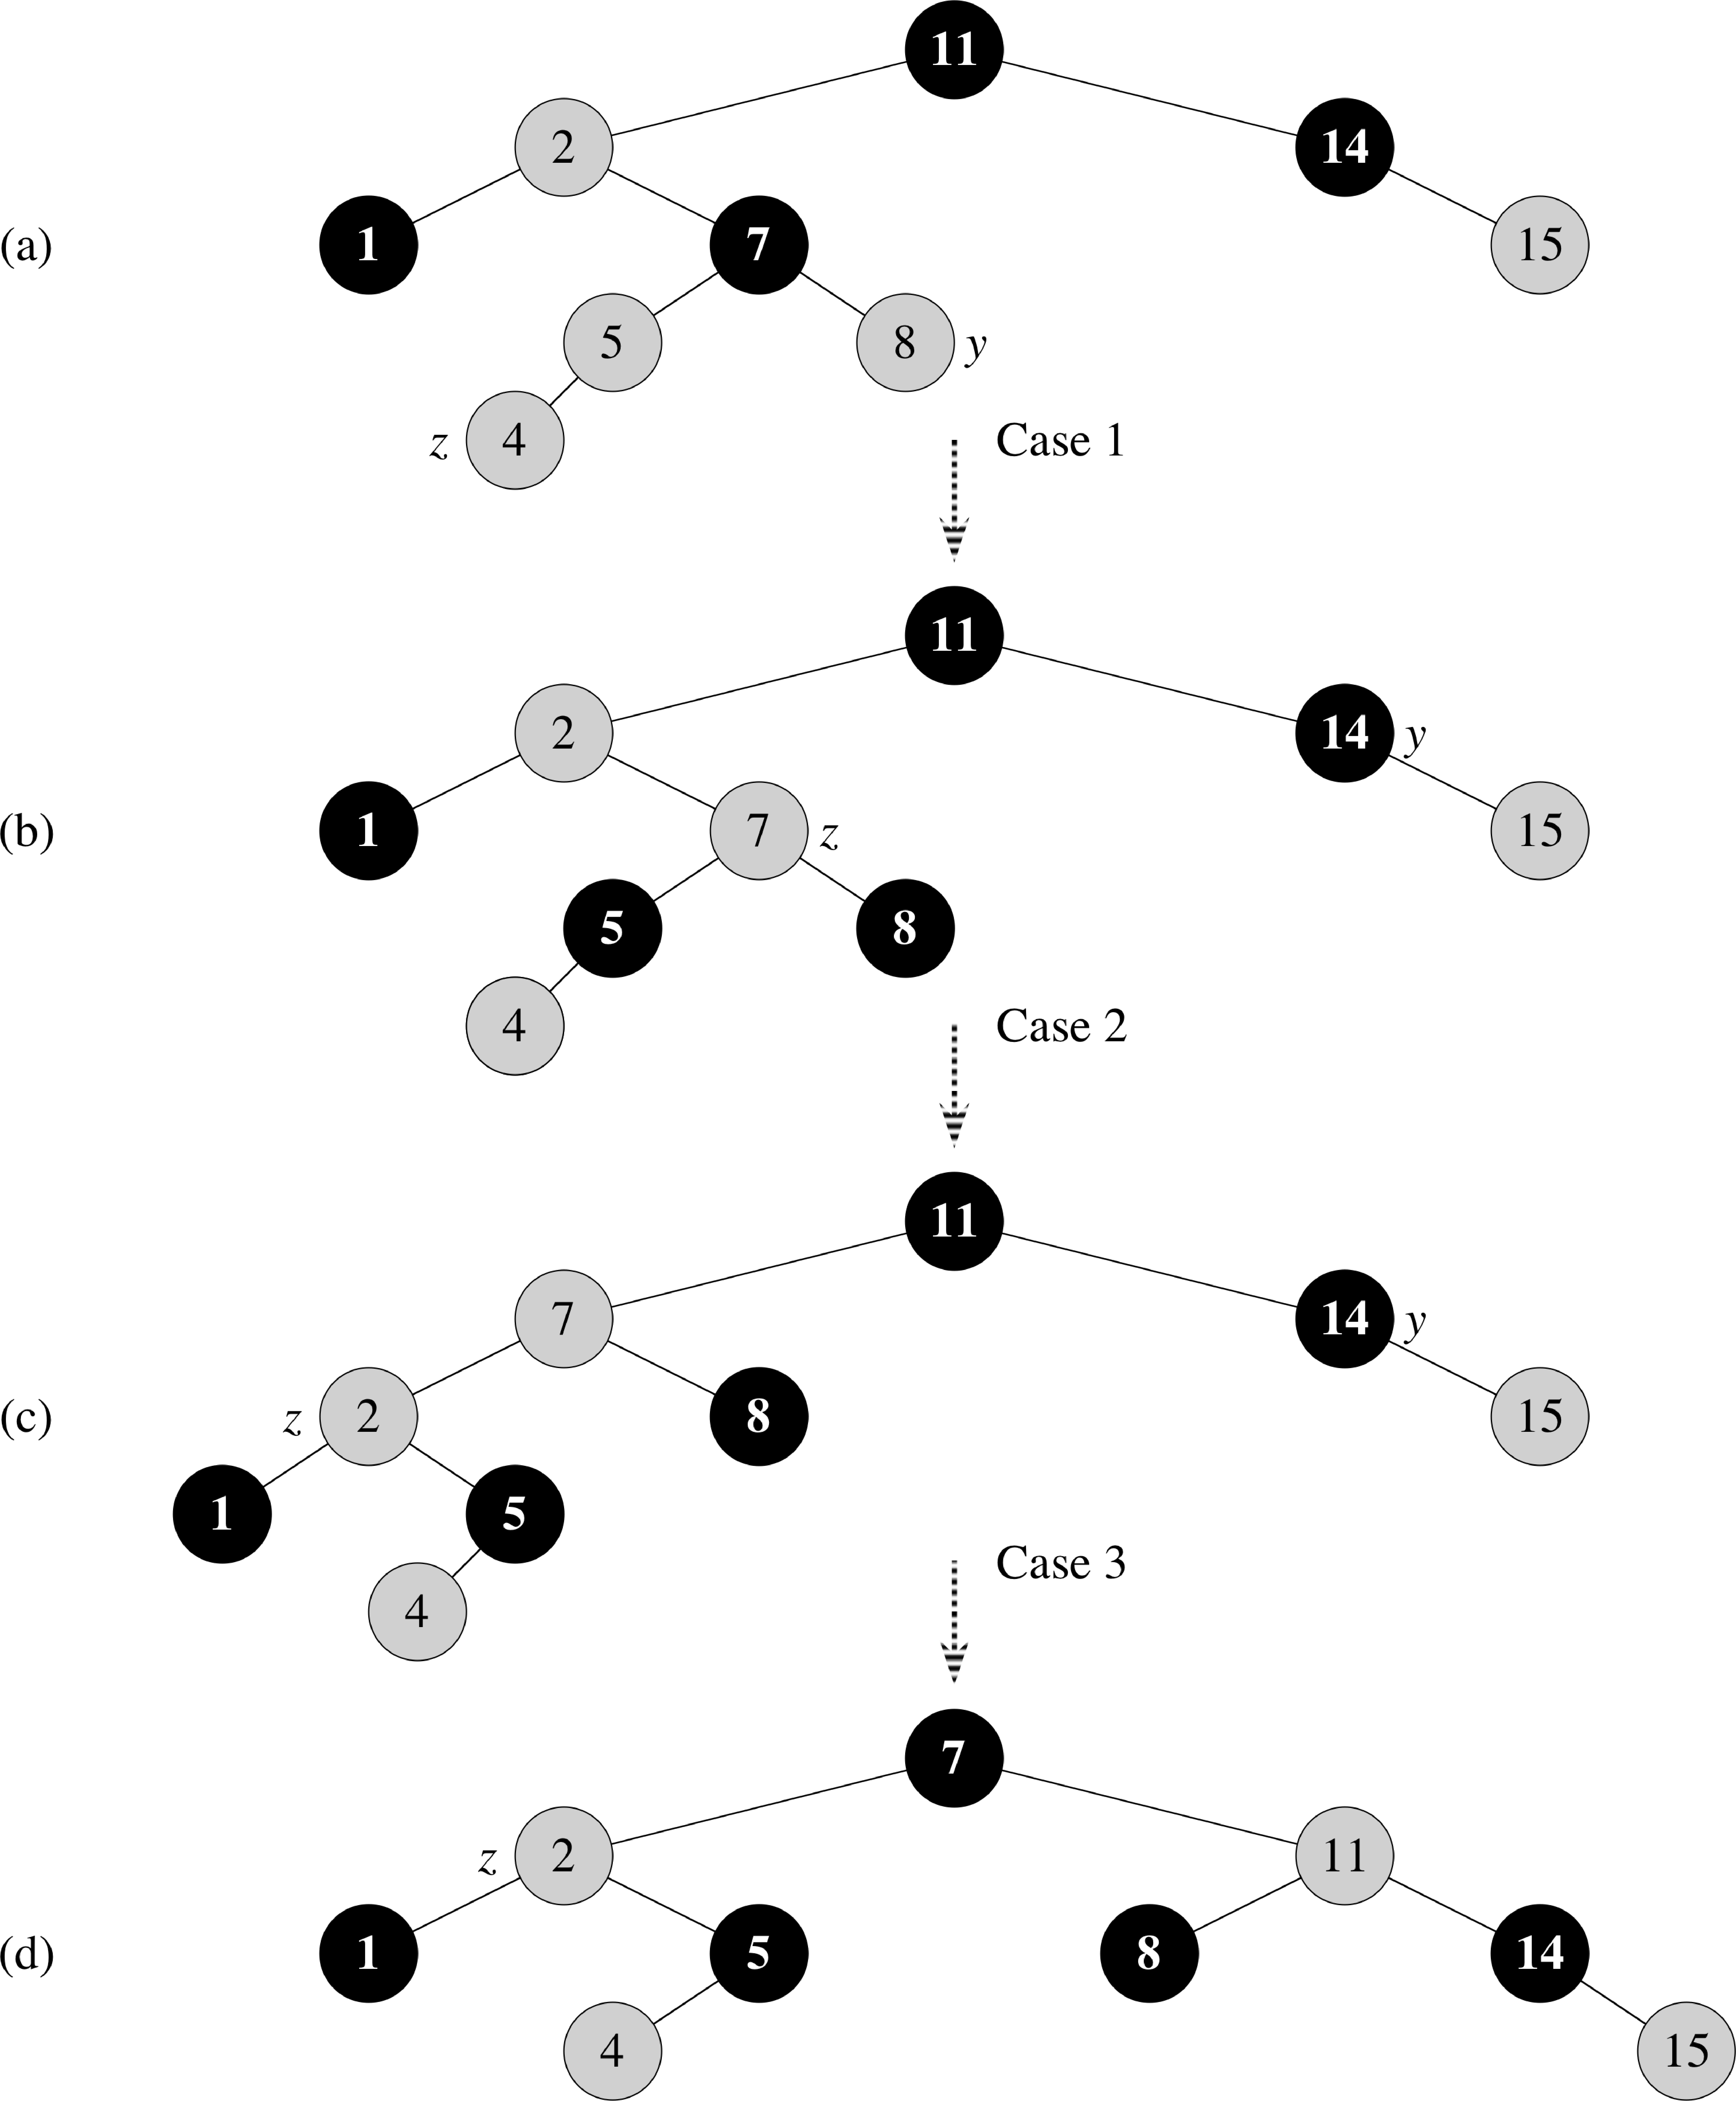
\includegraphics[height=0.8\textheight]{Fig-13-4.pdf}

\end{frame}

\sect{Insert fixup loop invariant.}
\bi
\ii $z$ is red
\ii There is at most one red-black violation:
\bi
\ii $z$ is a red root.
\ii $z$ and $\attrib{z}{p}$ are both red.
\ei
\ei

\end{frame}

\sect{Parent is red and  uncle is red:}

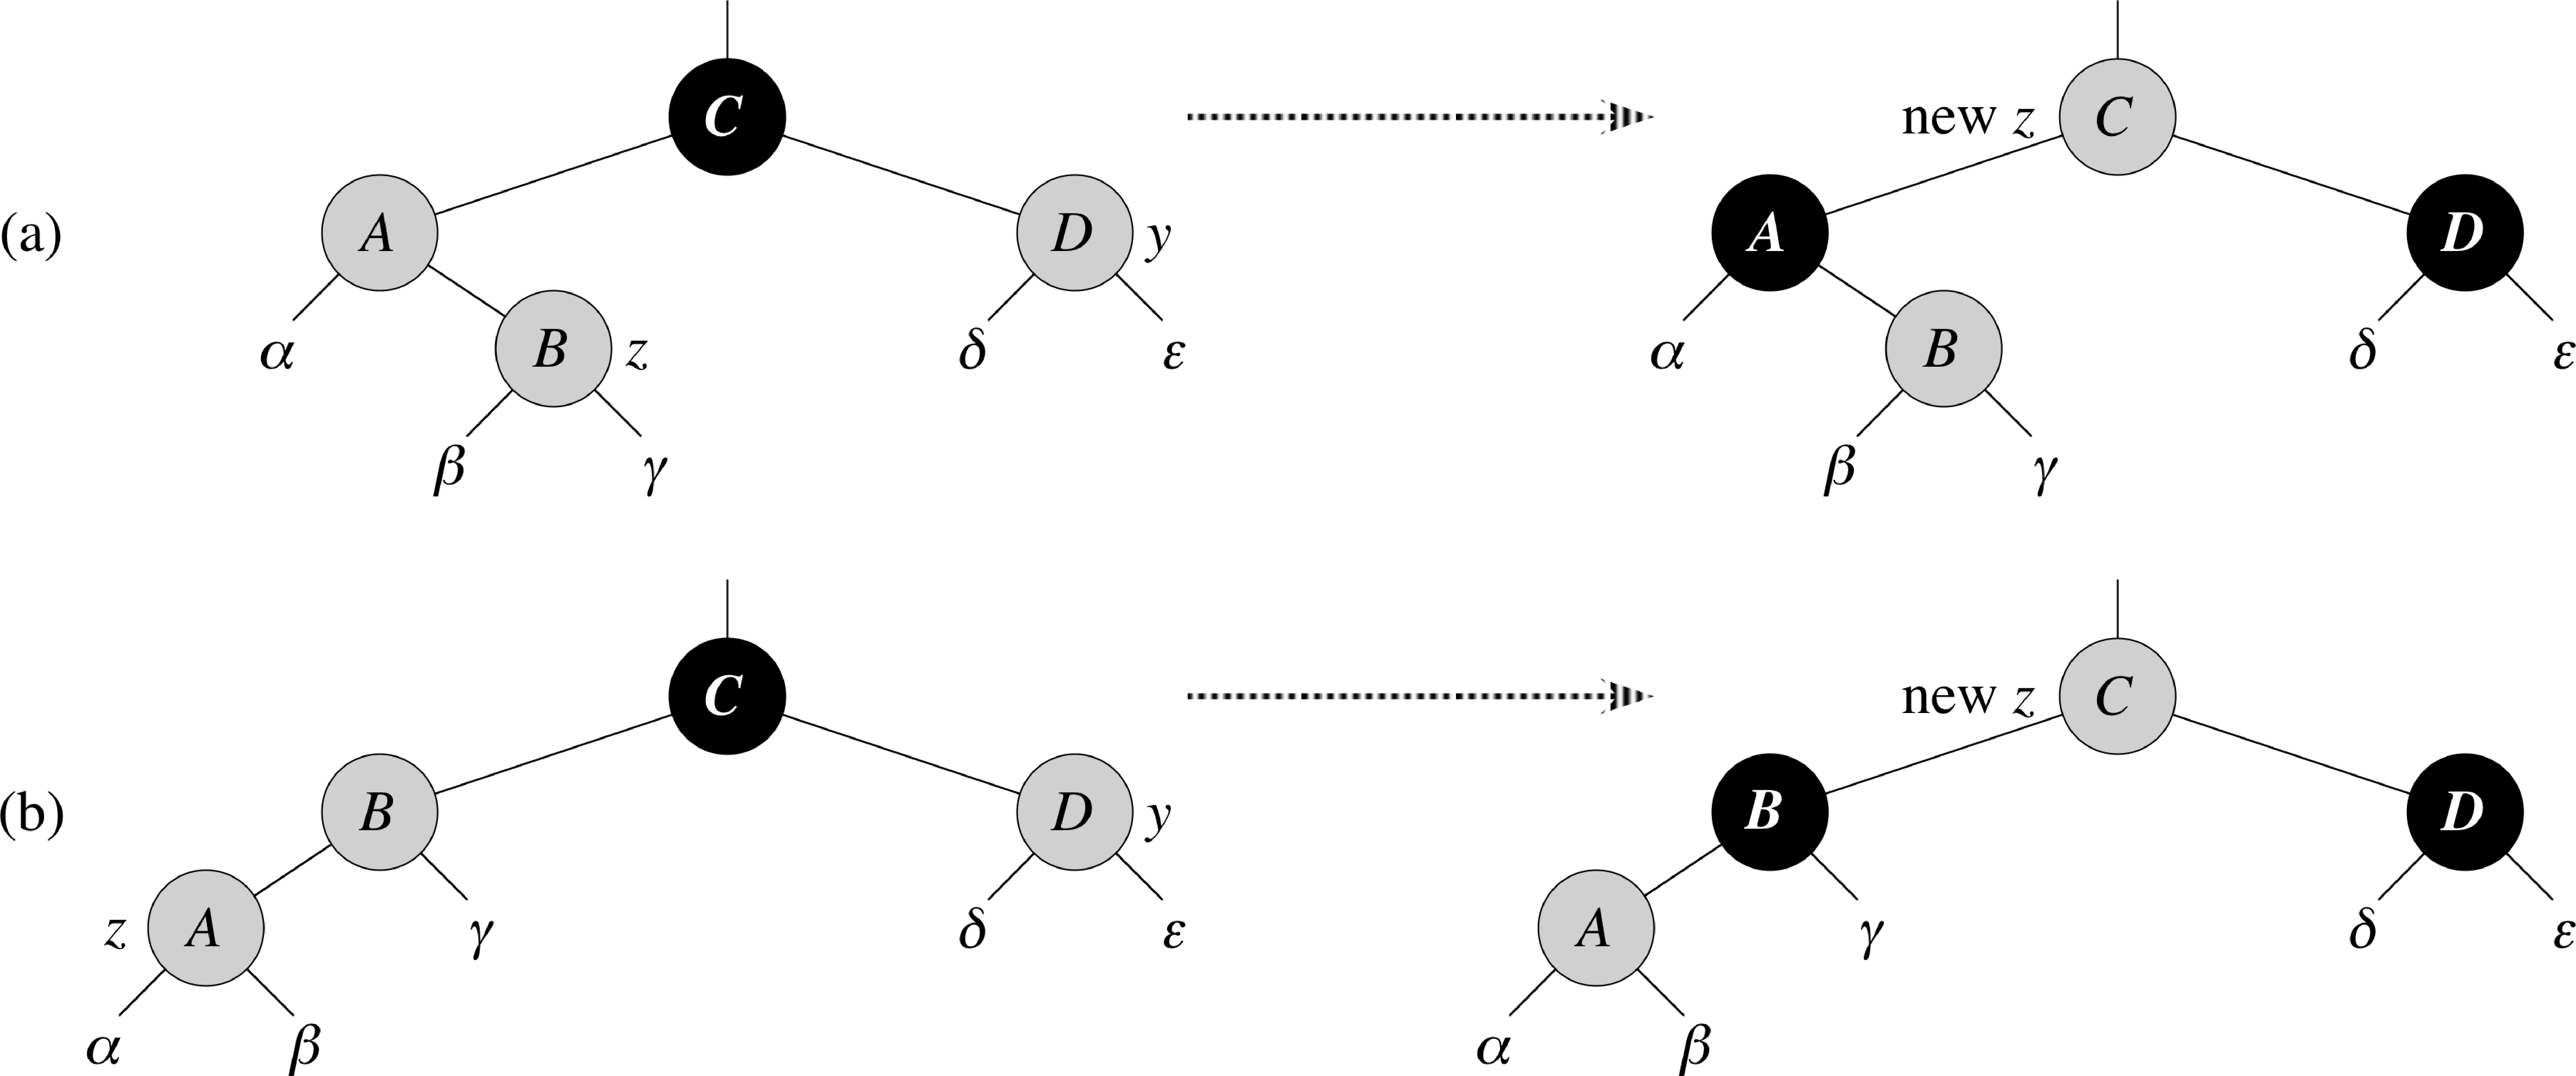
\includegraphics[width=\textwidth]{Fig-13-5.pdf}

\end{frame}

\sect{Parent is red and  uncle is black:}

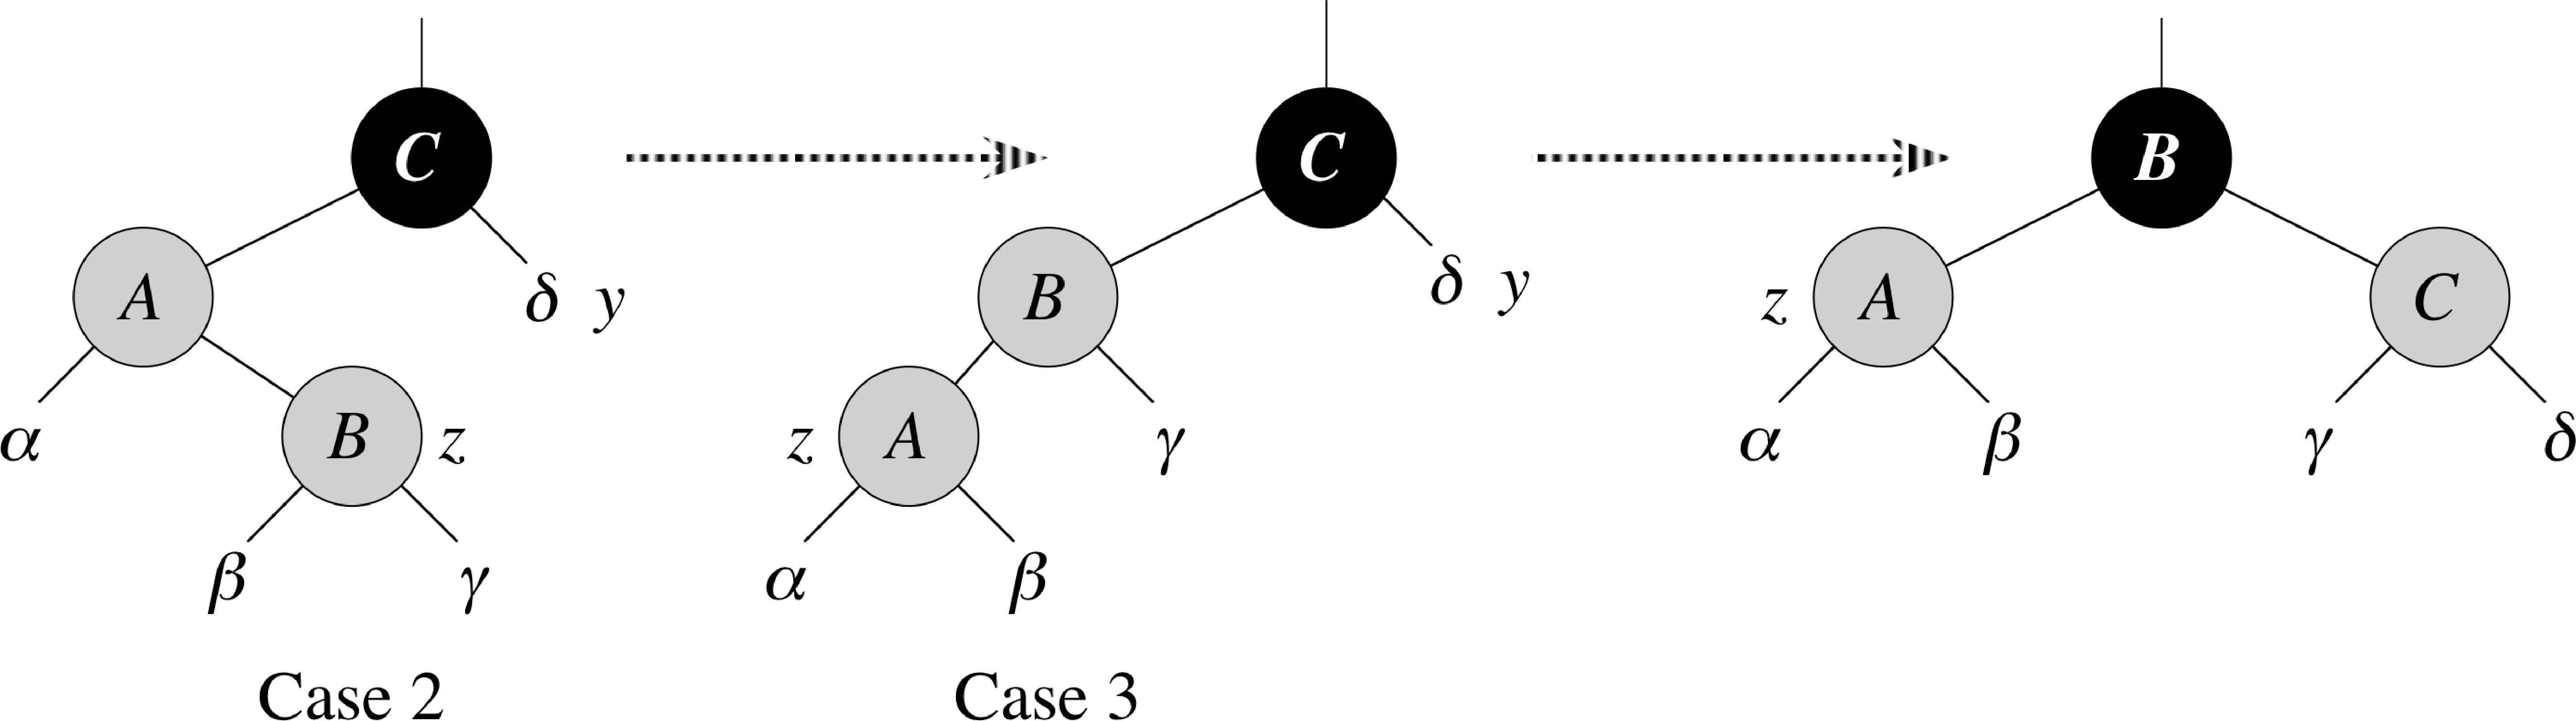
\includegraphics[width=\textwidth]{Fig-13-6.pdf}

\end{frame}

\sect{Analysis}
\bi
\ii $O(\lg n)$ time to insert into binary tree.
\ii Fixup also $O(\lg n)$:
\bi
\ii Each pass through the loop takes $O(1)$ time.
\ii Each iteration moves $z$ up two levels.
\ii $O(\lg n)$ levels.
\ii Also note that there are at most 2 rotations overall.
\ei
\ii Insertion into red-black tree is $O(\lg n)$.
\ei

\end{frame}

\sect{Deletion}

\bi\ii Not covered here.
\ii But also $O(\lg n)$.
\ei


  \begin{codebox}
  \Procname{$\proc{RB-Delete}(T,z)$}
  \li $ y \gets z $
  \li $\id{y-original-color} \gets \attrib{y}{color}$
  \li \If $\att{z}{left} \isequal \att{T}{nil}$  \Do
  \li $x \gets \att{z}{right}$
  \li $\proc{RB-Transplant}(T,z,\att{z}{right}$
  \end{codebox}

\end{frame}
%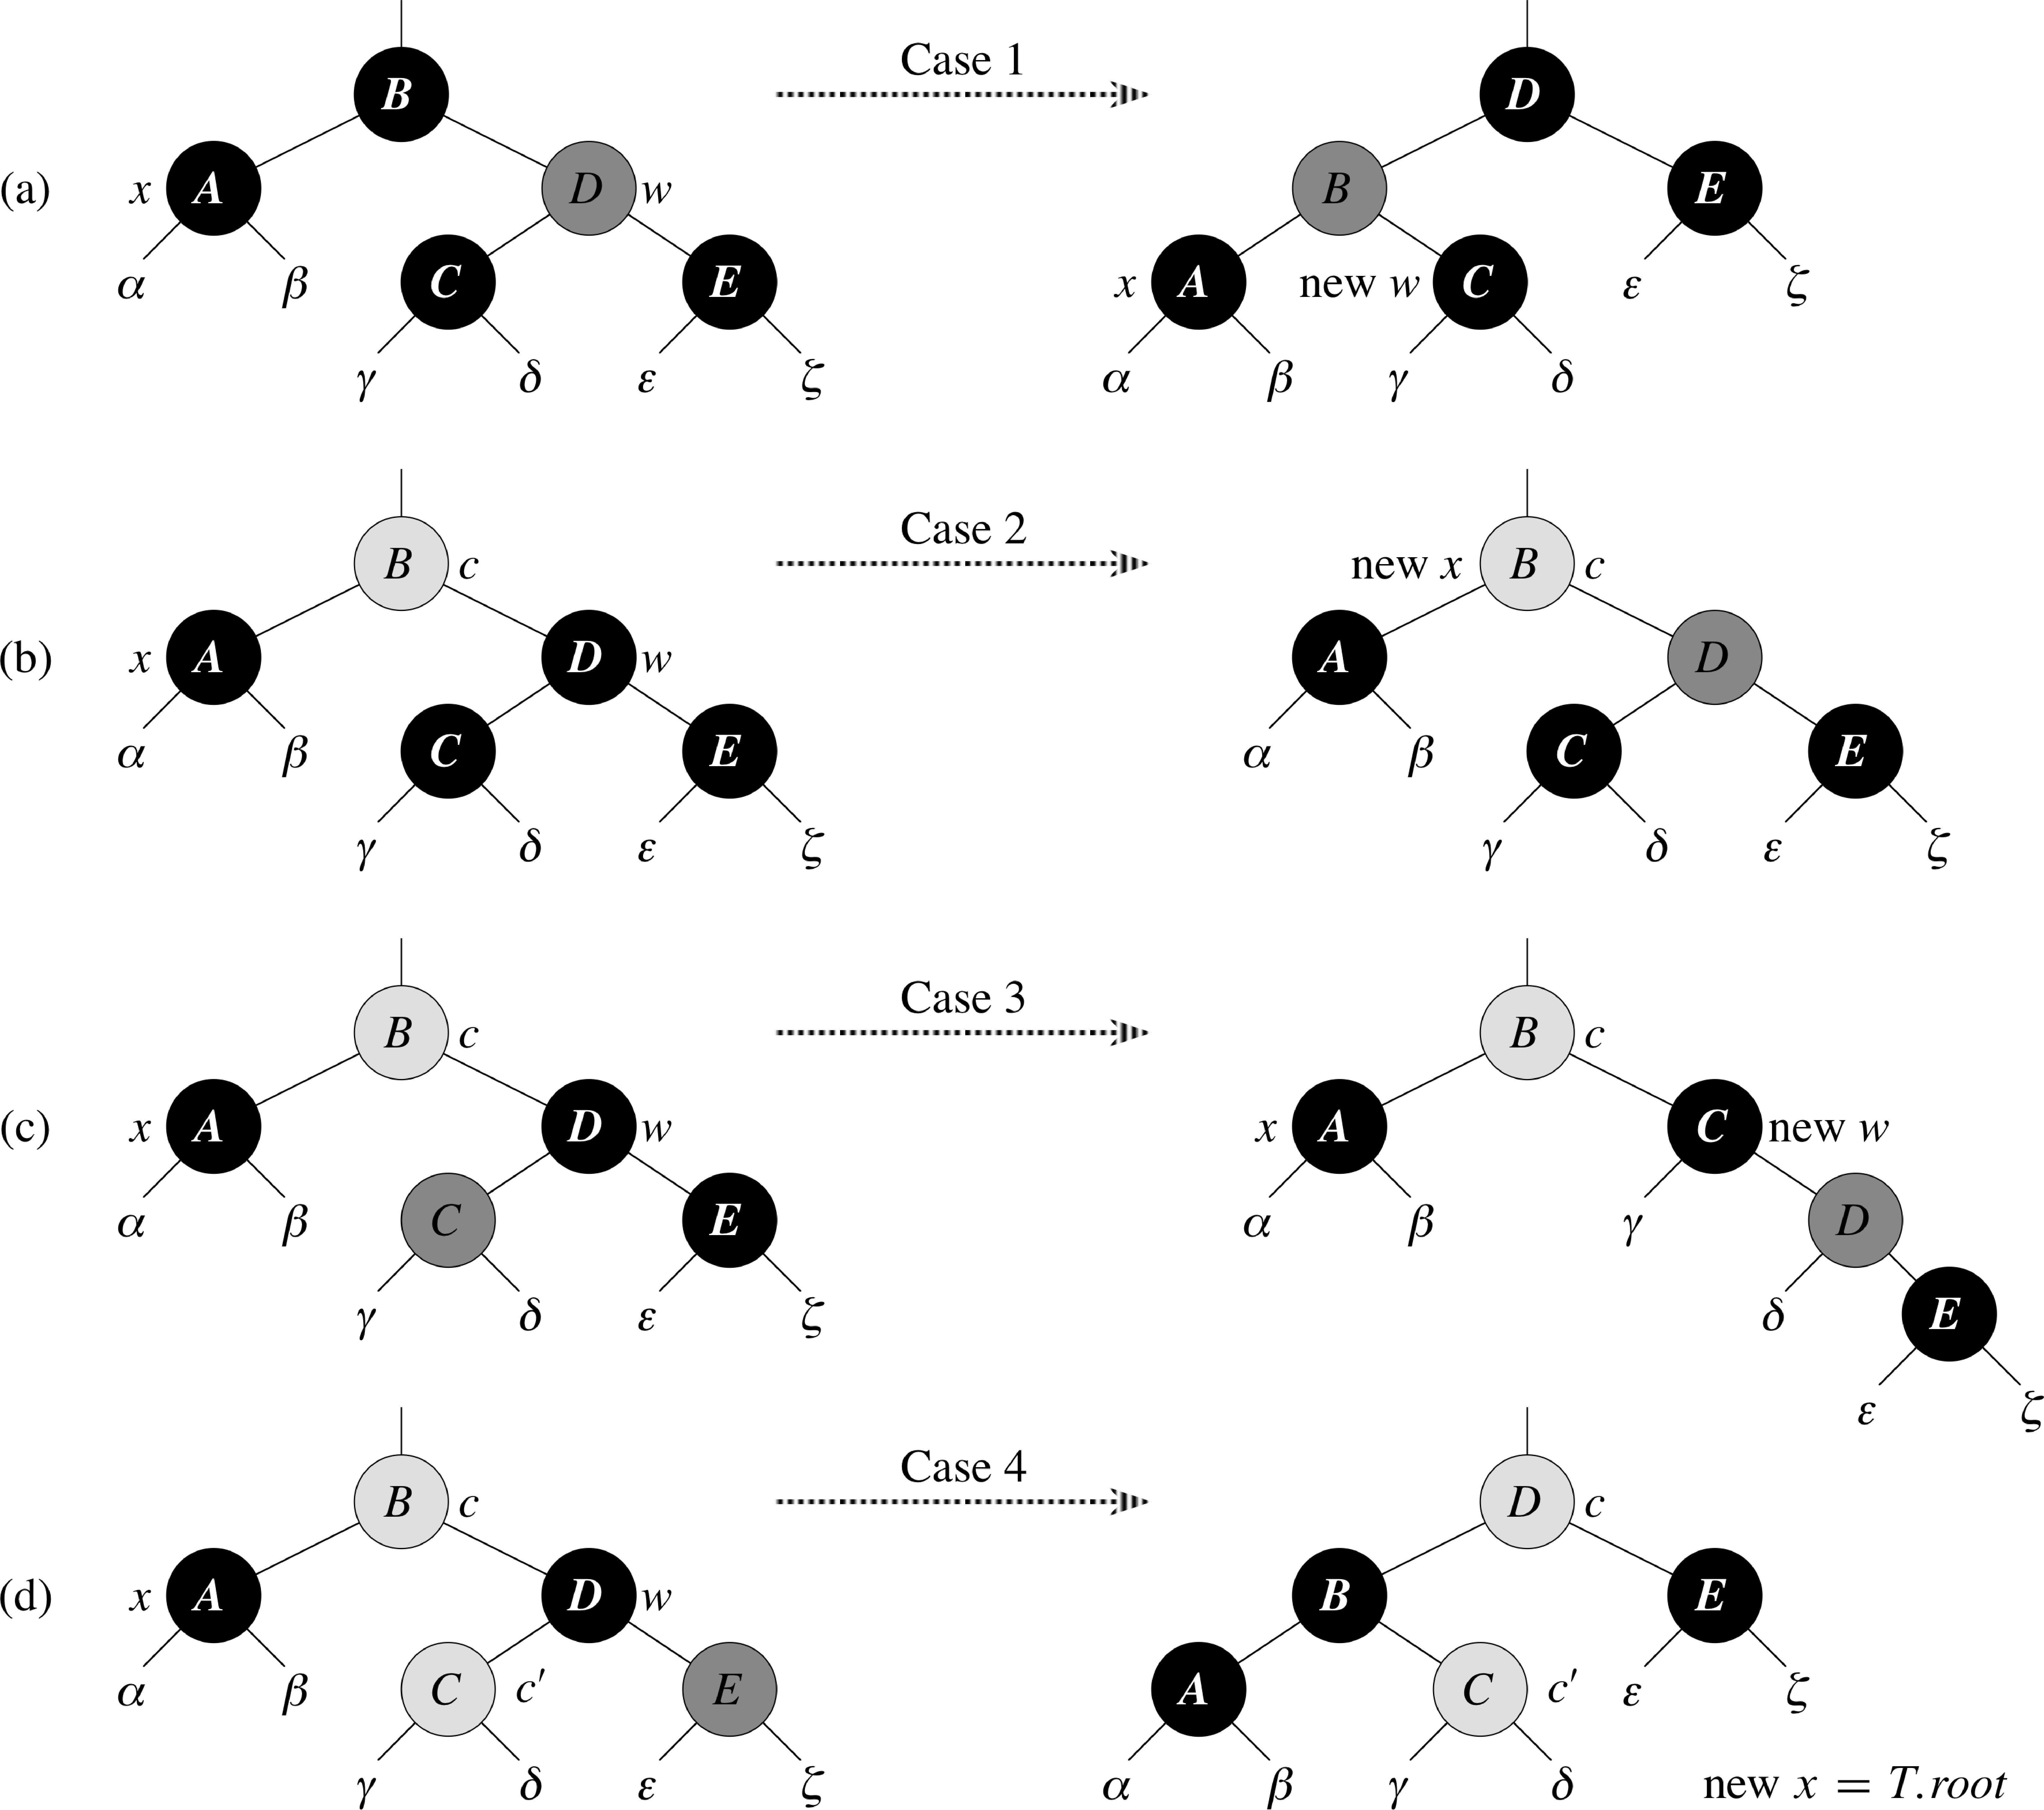
\includegraphics[width=\textwidth]{Fig-13-7.pdf}
%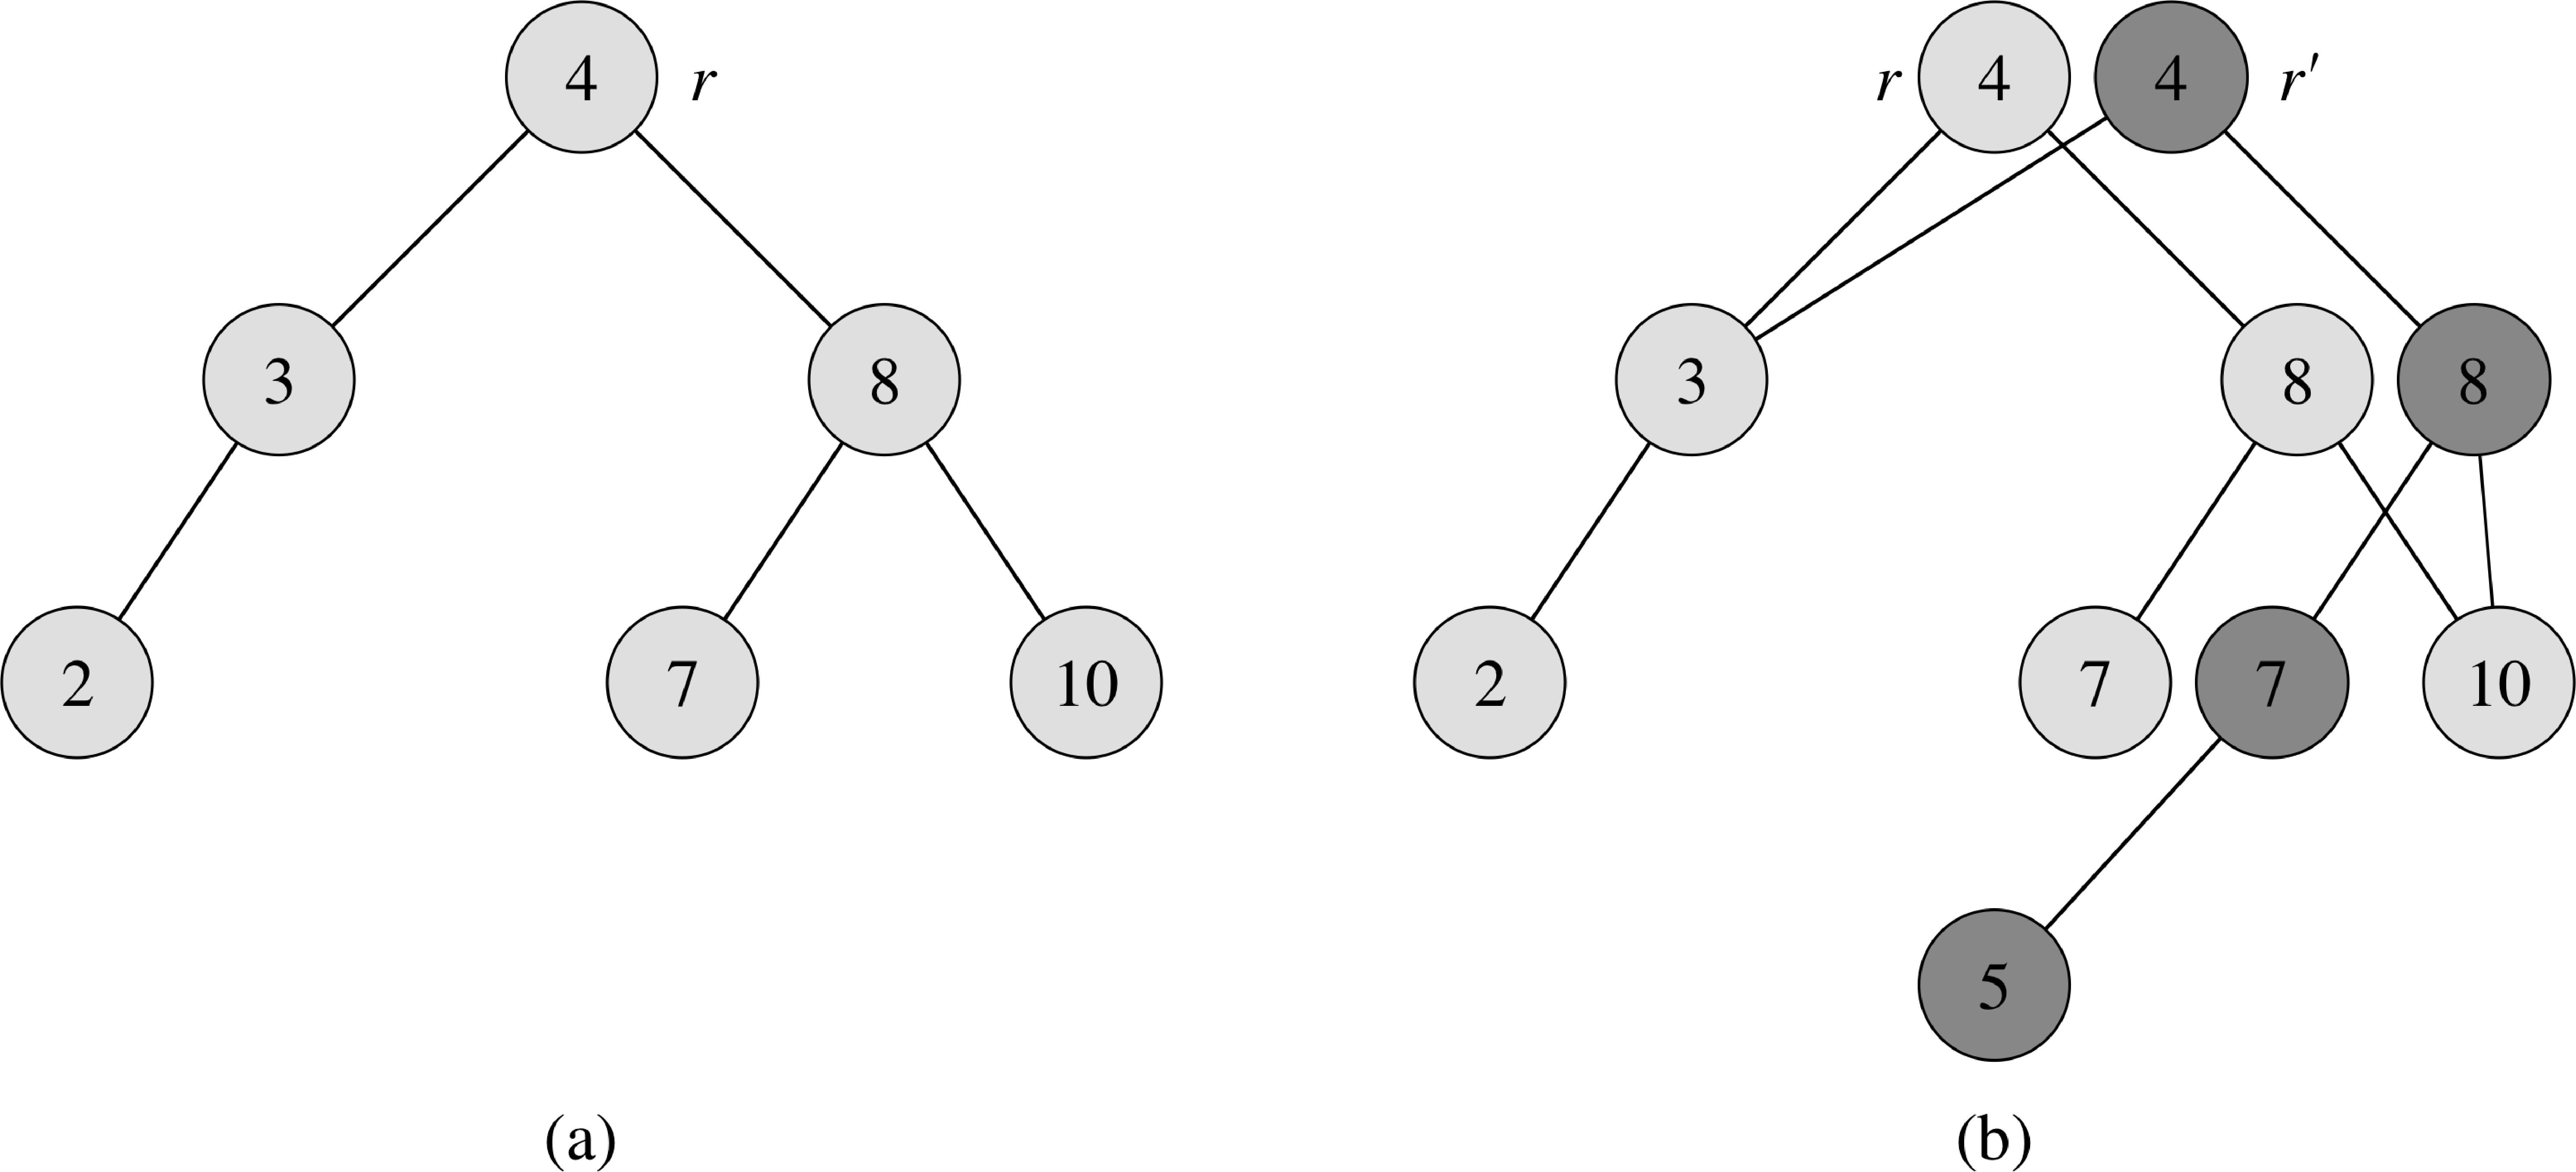
\includegraphics[width=\textwidth]{Fig-13-8.pdf}
%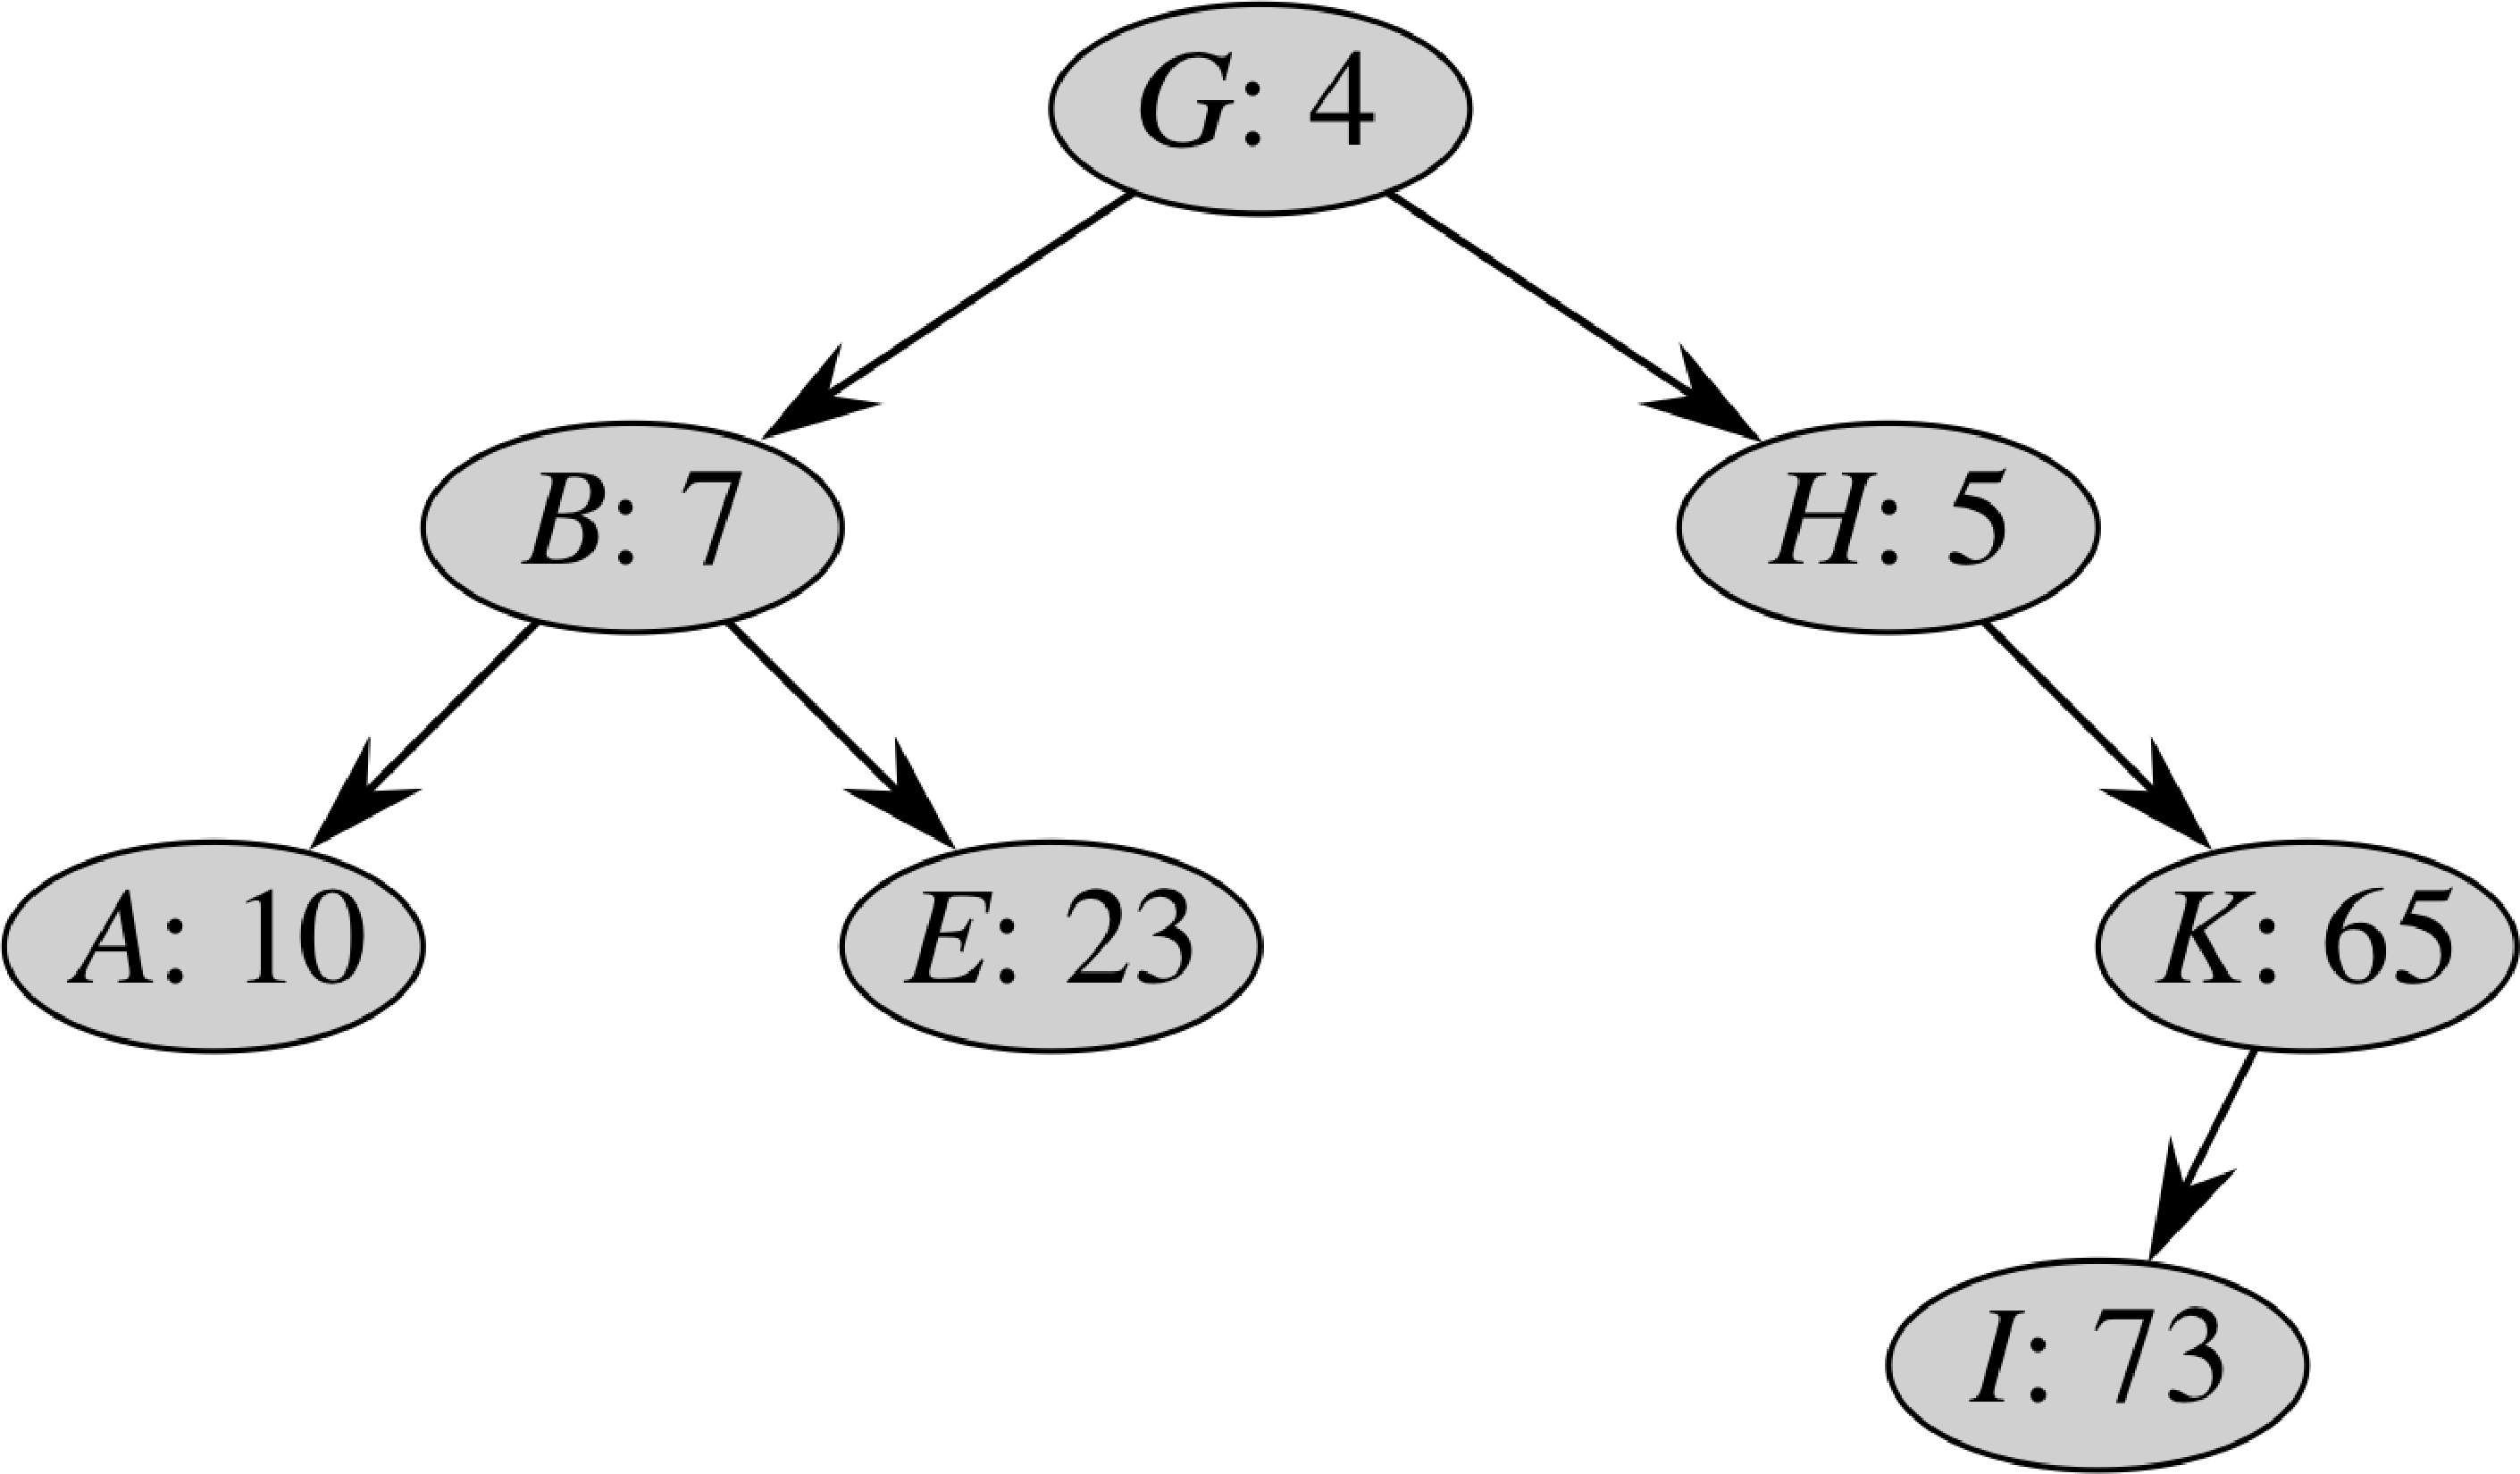
\includegraphics[width=\textwidth]{Fig-13-9.pdf}

\end{document}
